\documentclass[twocolumn]{article}
\usepackage{graphicx}
\usepackage[utf8]{inputenc}
\usepackage[a4paper, margin=0.79in]{geometry}
\usepackage{lastpage}
\usepackage[compact]{titlesec}
\usepackage{float}
\usepackage{microtype}
\usepackage{caption}
\captionsetup{font=scriptsize, labelfont=bf, skip=2pt}
\titleformat{\section}[hang]{\bfseries\large}{\thesection}{0.5em}{}
\titleformat{\subsection}[hang]{\bfseries\normalsize}{\thesubsection}{0.5em}{}
\setlength{\textfloatsep}{4pt plus 1pt minus 1pt}
\setlength{\floatsep}{3pt plus 1pt minus 1pt}
\setlength{\intextsep}{3pt plus 1pt minus 1pt}
\setlength{\abovecaptionskip}{2pt}
\setlength{\belowcaptionskip}{0pt}
\setlength{\parskip}{1pt}
\title{\large{\textbf{Wireless IoT and LAN (CESE4060): Matlab or NS3 Report}}}
\author{
    \small Tobias Veselka (4451848, tobiasveselka1) \and
    \small Enes Kaya (5279003, ekaya)
}
\date{\today}
\begin{document}
\maketitle
\begin{center}
    \footnotesize{Report contains \pageref{LastPage} of maximum 4 pages.}
\end{center}

% =========================================================================
\section{Basic Idea}
% =========================================================================

This work evaluates \textbf{IEEE 802.11ac} (Wi-Fi~5, TDMA) and
\textbf{IEEE 802.11ax} (Wi-Fi~6, OFDMA) through two system-level scenarios
simulated in MATLAB. The core architectural difference is the multiple-access
scheme: 802.11ac grants the full 80~MHz channel to one user at a time in
round-robin, while 802.11ax divides it into four simultaneous 20~MHz Resource
Units (RUs), one per user~\cite{khorov2019}.

The intuition is that TDMA excels when all users share similar channel
conditions and large payloads, as no bandwidth is lost to sub-band splitting.
OFDMA excels when users differ in payload size or SNR, since each is served
independently and head-of-line blocking is eliminated~\cite{bellalta2016}.
\textbf{Scenario~A} stresses the delay behaviour with mixed large/small
payloads; \textbf{Scenario~B} stresses capacity and fairness with asymmetric
SNR (Near vs.\ Far users).

% =========================================================================
\section{Implementation}
% =========================================================================

All scripts use MATLAB's WLAN Toolbox with LDPC coding, TGax Model-B fading
channel, CBW80 (80~MHz), and 50 packets per user. Four independent
\texttt{wlanTGaxChannel} objects are created at distances \{3,~5,~7,~9\}~m.

\textbf{Traffic profiles.}
Scenario~A: two Video users (1500~B, MCS\textsubscript{ac}=8,
MCS\textsubscript{ax}=10, SNR=30~dB) and two Voice users (128~B,
MCS\textsubscript{ac}=4, MCS\textsubscript{ax}=5, SNR=25~dB).
Scenario~B: two Near users (1024~B, MCS\textsubscript{ac}=9,
MCS\textsubscript{ax}=11, SNR=38/34~dB) and two Far users (512~B,
MCS\textsubscript{ac}=2--1, MCS\textsubscript{ax}=3--2, SNR=12/8~dB).

\textbf{802.11ac (TDMA).}
Each user is simulated with \texttt{wlanVHTConfig} (CBW80). The slot
duration is measured from the waveform length divided by the sample rate.
In round-robin, per-user throughput is $\eta_u = G_u / (T_u \times N)$,
where $N=4$ users share the channel time. The packet delay for user~$u$
(position $u$ in the round) is modelled as:
\textit{queuing} $= (u-1) \times T_u$ (uses the user's own slot duration
as a proxy for all preceding slots), plus its own transmission time~$T_u$,
plus propagation delay $d_u/c$.

\textbf{802.11ax (HE-SU workaround).}
\texttt{wlanHEMUConfig} cannot be used for SISO chains because
\texttt{NumSpaceTimeStreams} is read-only in multi-RU configurations and
always defaults to a value exceeding the number of transmit antennas, causing
a fatal error. The workaround simulates each user independently with
\texttt{wlanHESUConfig} (CBW80, SISO). The OFDMA simultaneity is captured
through time accounting: the shared PPDU slot equals the longest of all
users' HE-SU frame durations (\texttt{ofdma\_slot = max(slot\_dur\_ax)}).
All users are charged this same clock duration per packet round, which is
physically correct since in 802.11ax DL-OFDMA the AP transmits all RUs
simultaneously and the frame length is set by the slowest RU. For 802.11ax,
packet delay is \textit{ofdma\_slot}~$+$~$d_u/c$ (no queuing).

\textbf{Spectral efficiency.}
Network-level SE divides total throughput by 80~MHz for both standards.
Per-user SE for 802.11ax is referenced to the 20~MHz sub-band
(\texttt{BW\_HZ/N\_USERS}); for 802.11ac it uses the full 80~MHz.

\textbf{Metrics.}
Total and per-user throughput (Mbps); average packet delay ($\mu$s);
network SE (bps/Hz); Jain's Fairness Index~\cite{jain1984}:
$J = (\sum x_i)^2 / (N \sum x_i^2)$; normalised per-user throughput share.

% =========================================================================
\section{Results}
% =========================================================================

\subsection*{Scenario A --- Heterogeneous Traffic (Small vs.\ Large Packets)}

\begin{figure}[H]
\centering
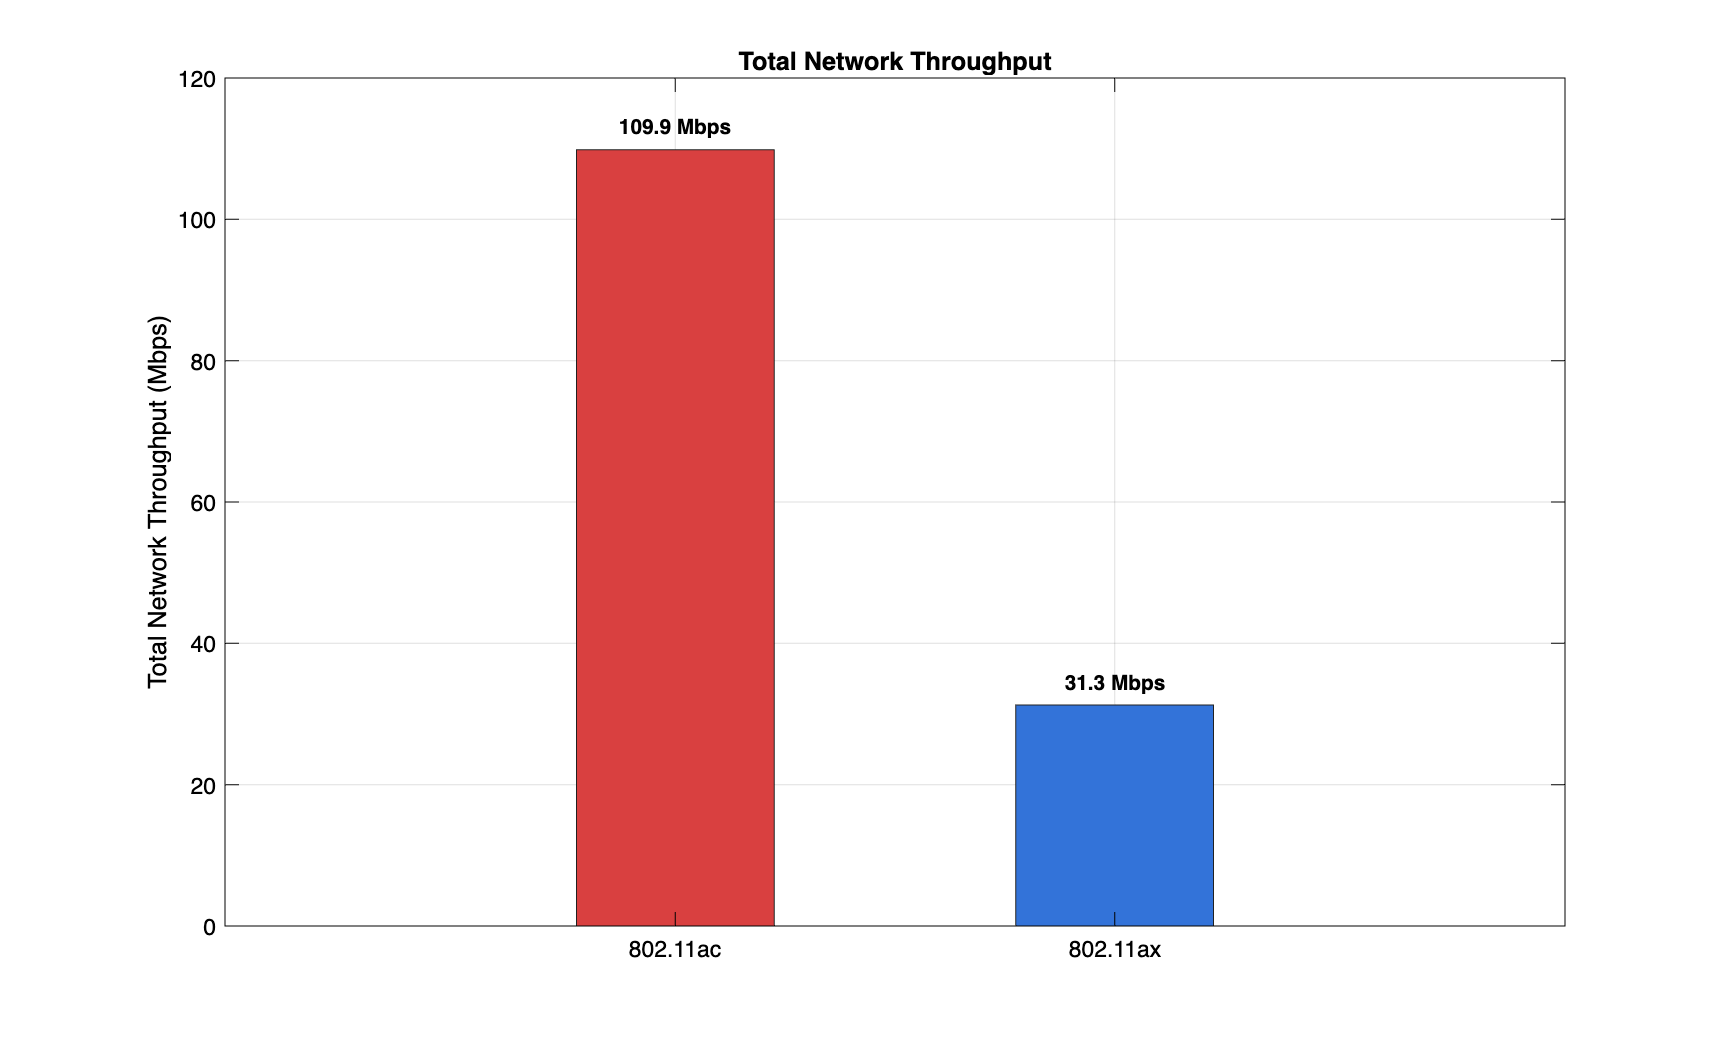
\includegraphics[width=\linewidth]{figures/scenario-a/total_network_throughput.png}
\caption{Scenario~A: Total network throughput. 802.11ac (108.8~Mbps)
achieves roughly double 802.11ax (54.4~Mbps). Splitting the 80~MHz band into
four 20~MHz RUs with guard bands halves total capacity when all users have
high SNR.}
\label{fig:a_tot}
\end{figure}

\begin{figure}[H]
\centering
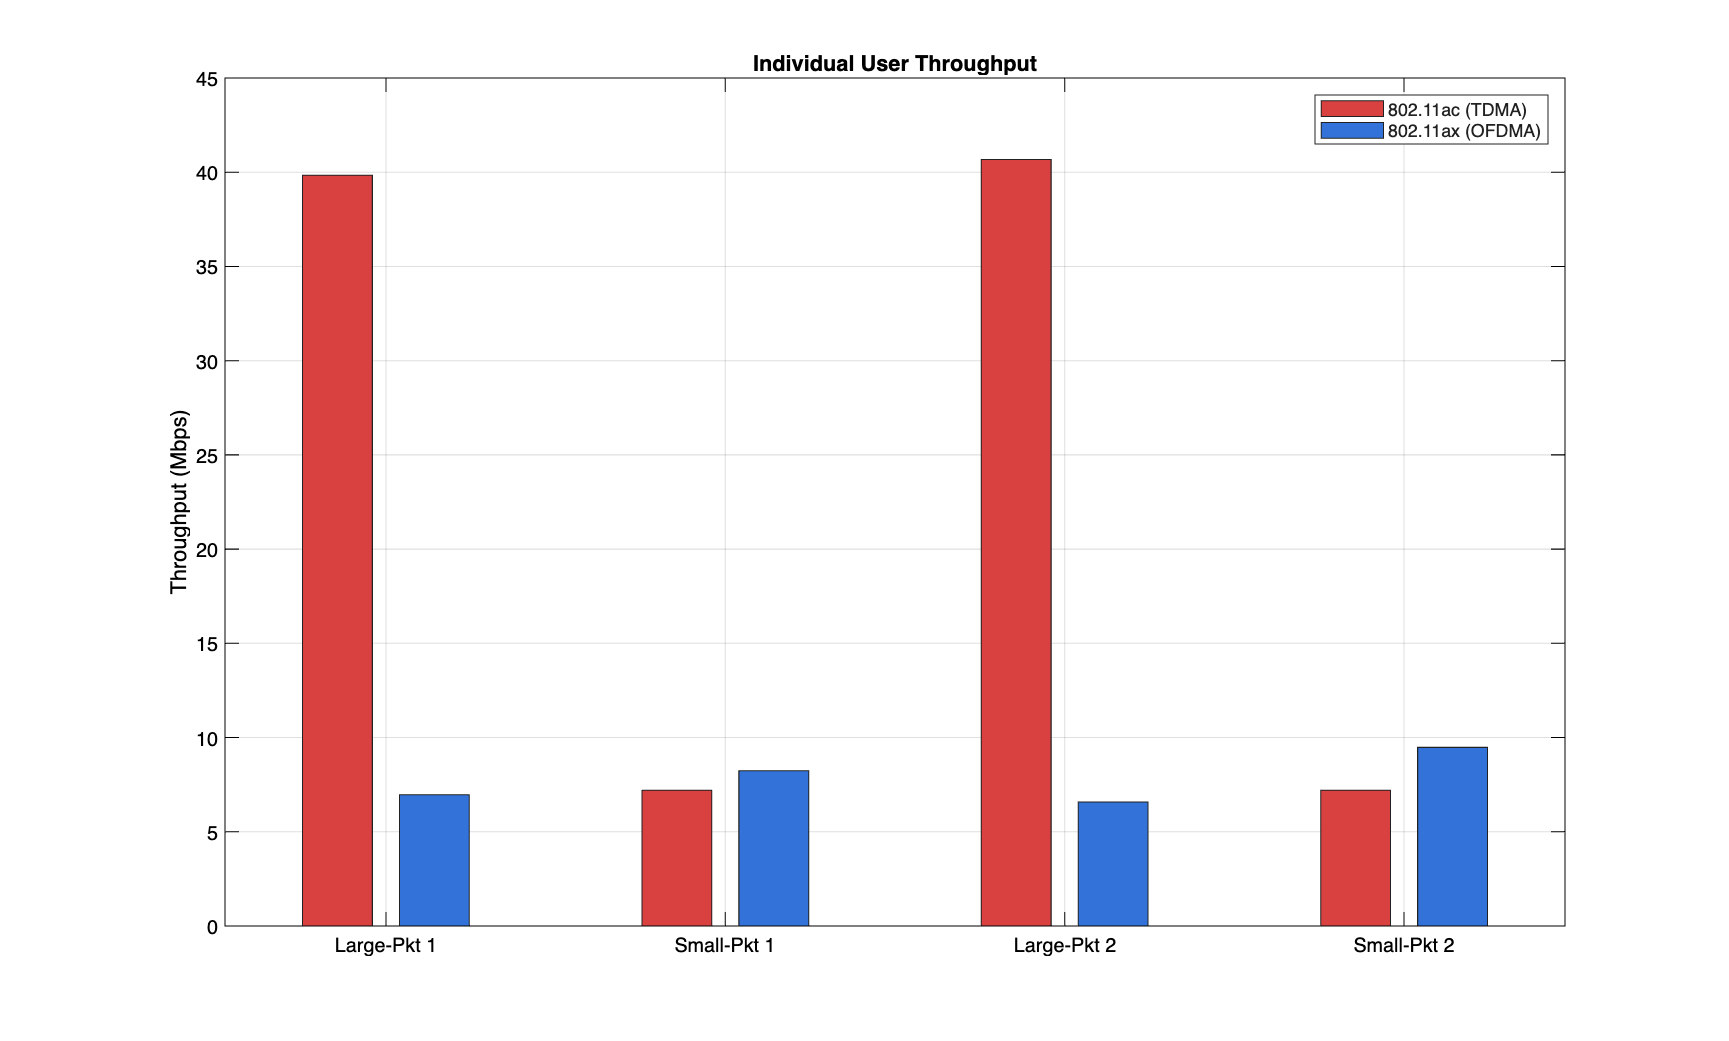
\includegraphics[width=\linewidth]{figures/scenario-a/individual_user_throughput.png}
\caption{Scenario~A: Per-user throughput. In 802.11ac, Large-Pkt users
dominate ($\approx$40~Mbps) while Small-Pkt users receive only $\approx$7~Mbps.
In 802.11ax the pattern reverses: Small-Pkt users reach $\approx$22.6~Mbps
in their dedicated 20~MHz RU, while Large-Pkt users fall to 3--6~Mbps.}
\label{fig:a_ind}
\end{figure}

\begin{figure}[H]
\centering
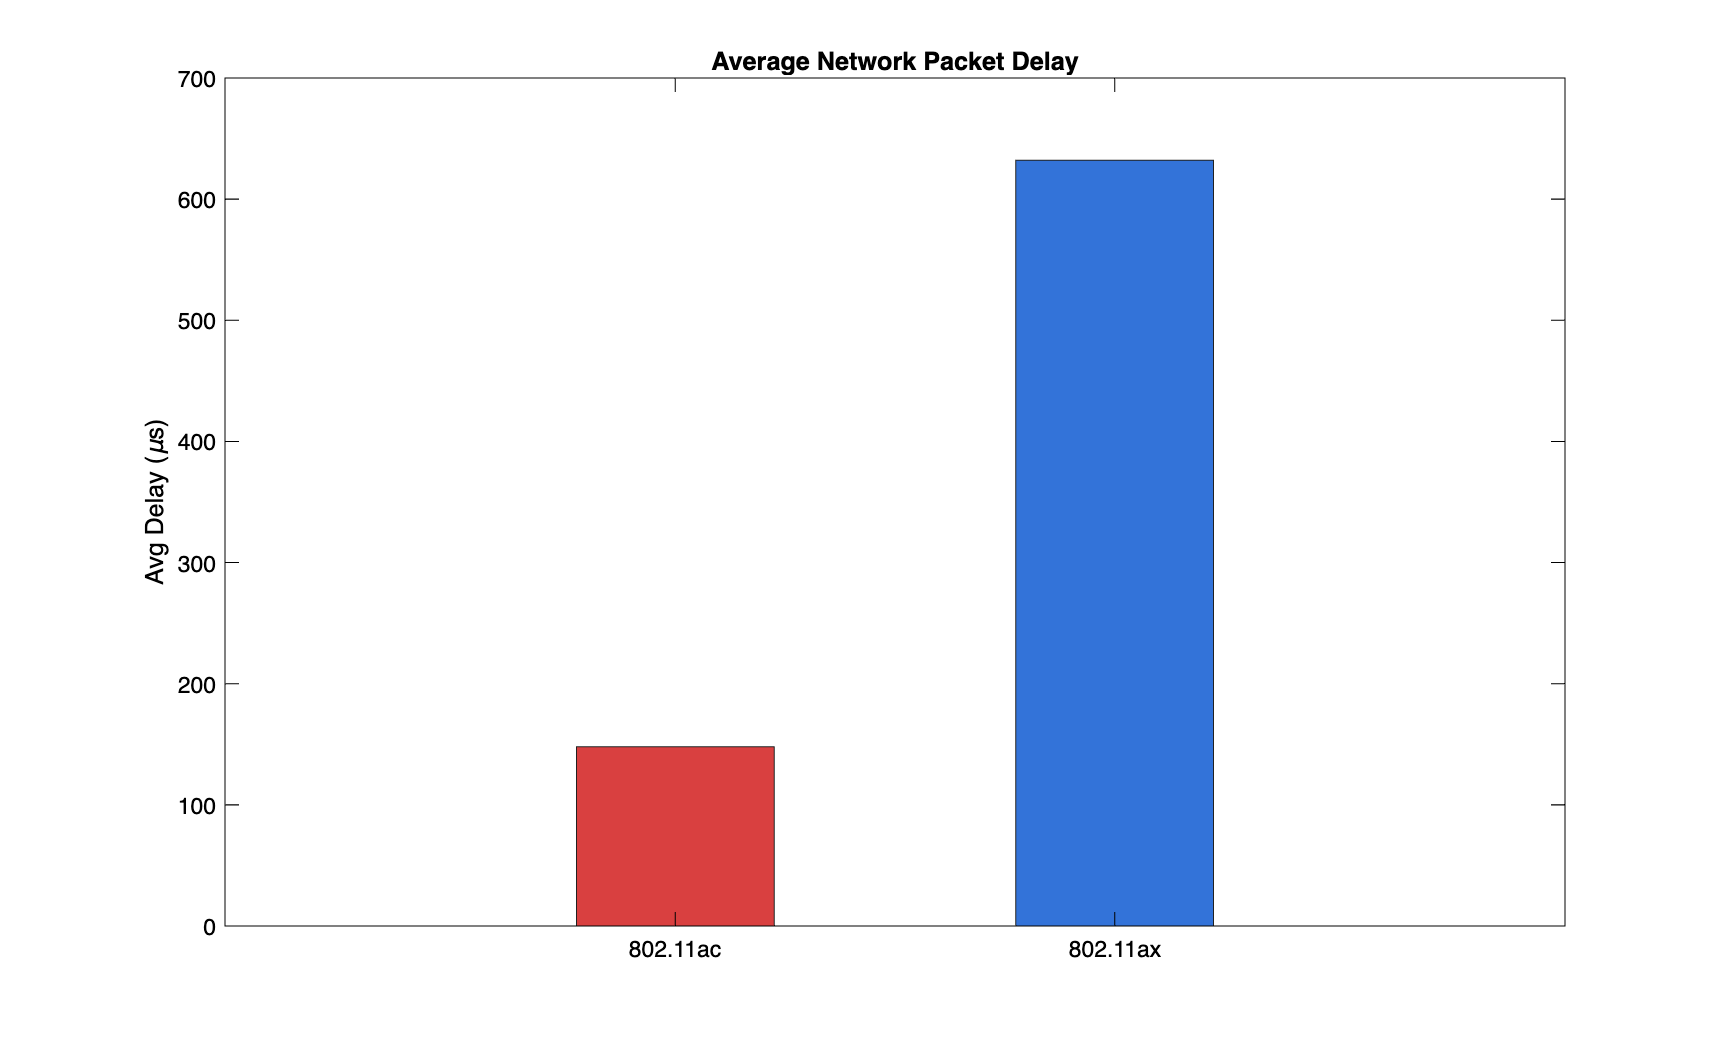
\includegraphics[width=\linewidth]{figures/scenario-a/net_delay.png}
\caption{Scenario~A: Average network packet delay. 802.11ax ($\approx$83~$\mu$s)
reduces network delay versus 802.11ac ($\approx$148~$\mu$s) by eliminating
queuing through parallel OFDMA scheduling.}
\label{fig:a_netdelay}
\end{figure}

\begin{figure}[H]
\centering
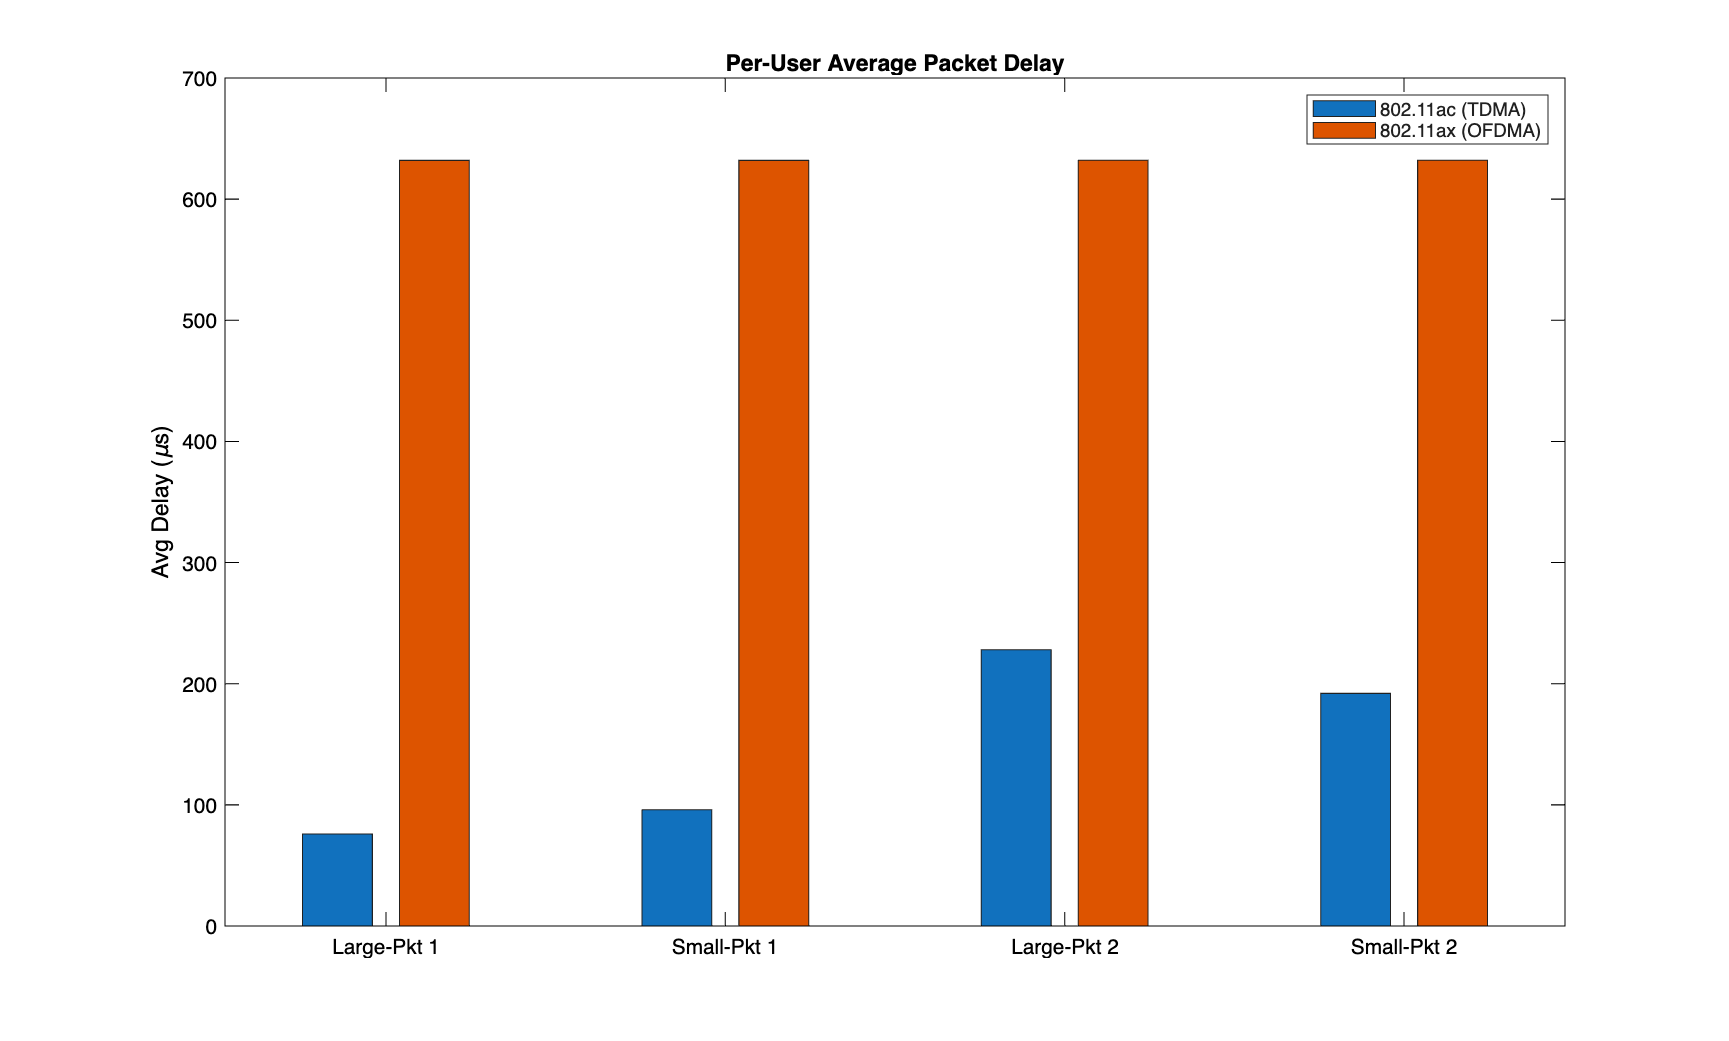
\includegraphics[width=\linewidth]{figures/scenario-a/user_delay.png}
\caption{Scenario~A: Per-user delay. 802.11ax enforces a uniform
$\approx$84~$\mu$s for every user. In 802.11ac, Large-Pkt~2 (position~3 in
round-robin) reaches 227~$\mu$s and Small-Pkt~2 (position~4) reaches
193~$\mu$s due to queuing.}
\label{fig:a_del}
\end{figure}

\begin{figure}[H]
\centering
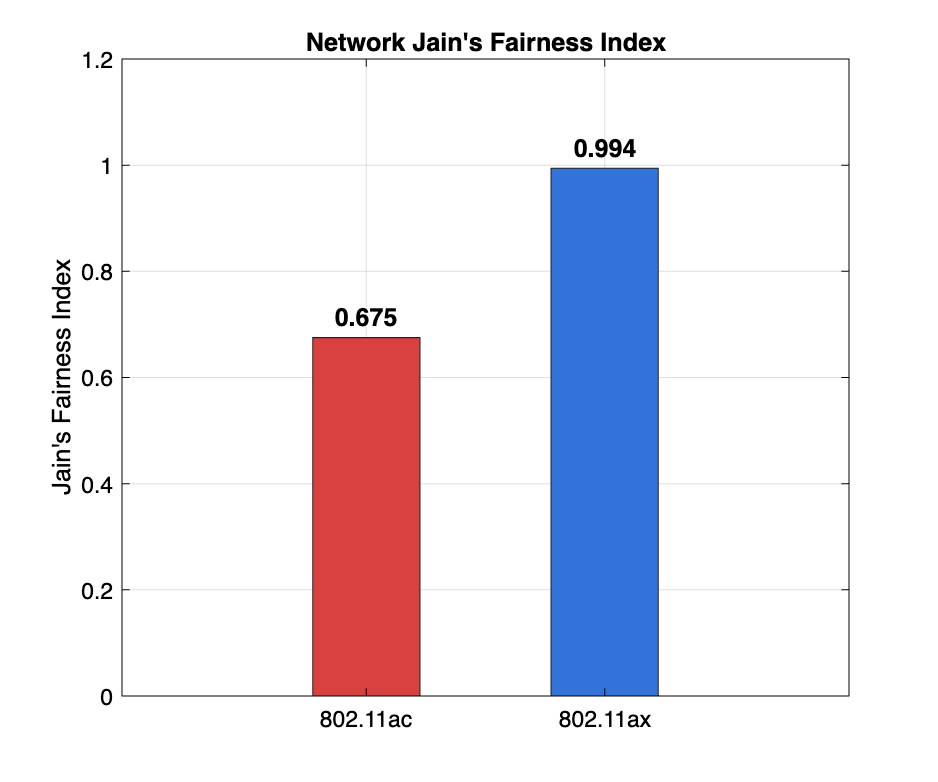
\includegraphics[width=\linewidth]{figures/scenario-a/jain_fairness_index.png}
\caption{Scenario~A: Jain's Fairness Index. 802.11ax (0.773) scores higher
than 802.11ac (0.675), because OFDMA distributes throughput more evenly
across traffic types.}
\label{fig:a_jain}
\end{figure}

\begin{figure}[H]
\centering
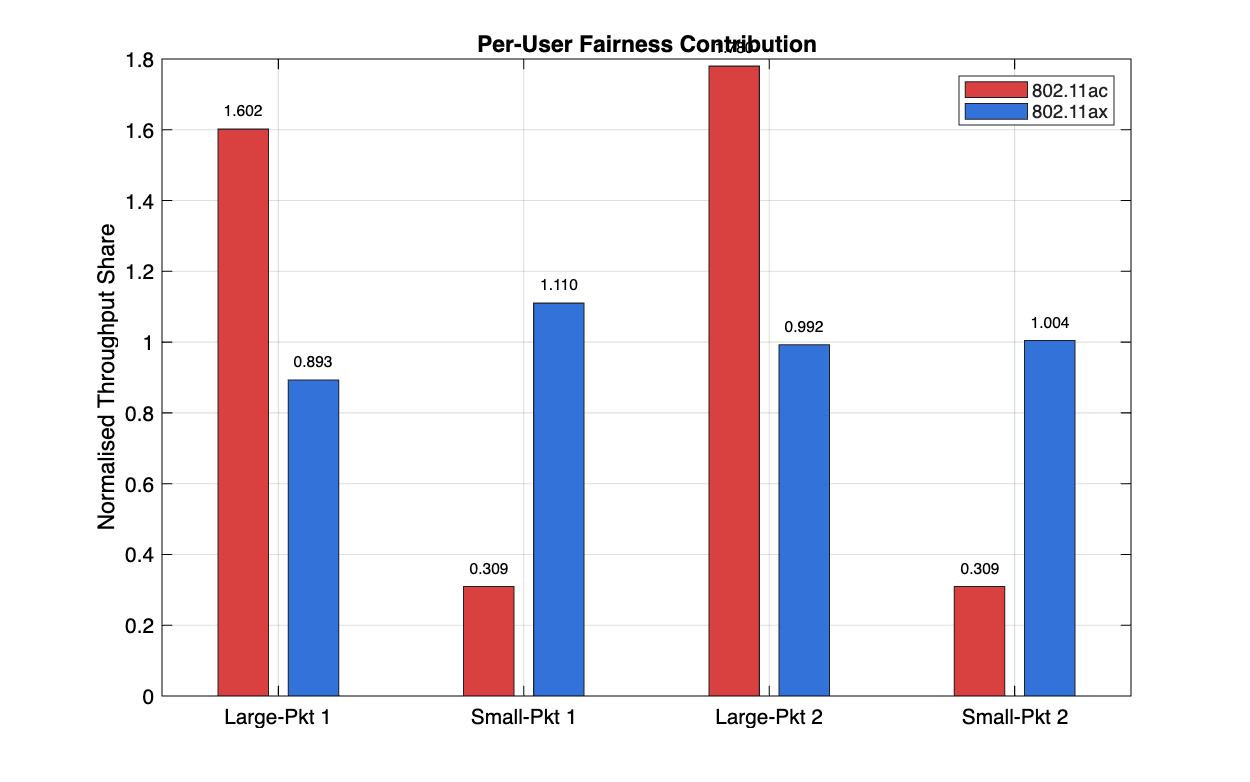
\includegraphics[width=\linewidth]{figures/scenario-a/user_fairness_contribution.png}
\caption{Scenario~A: Per-user normalised throughput share. In 802.11ac,
Large-Pkt users hold shares $>$1.6, while Small-Pkt users remain below
0.31. In 802.11ax, Small-Pkt users each reach 1.50, narrowing the
disparity.}
\label{fig:a_fair}
\end{figure}

\begin{figure}[H]
\centering
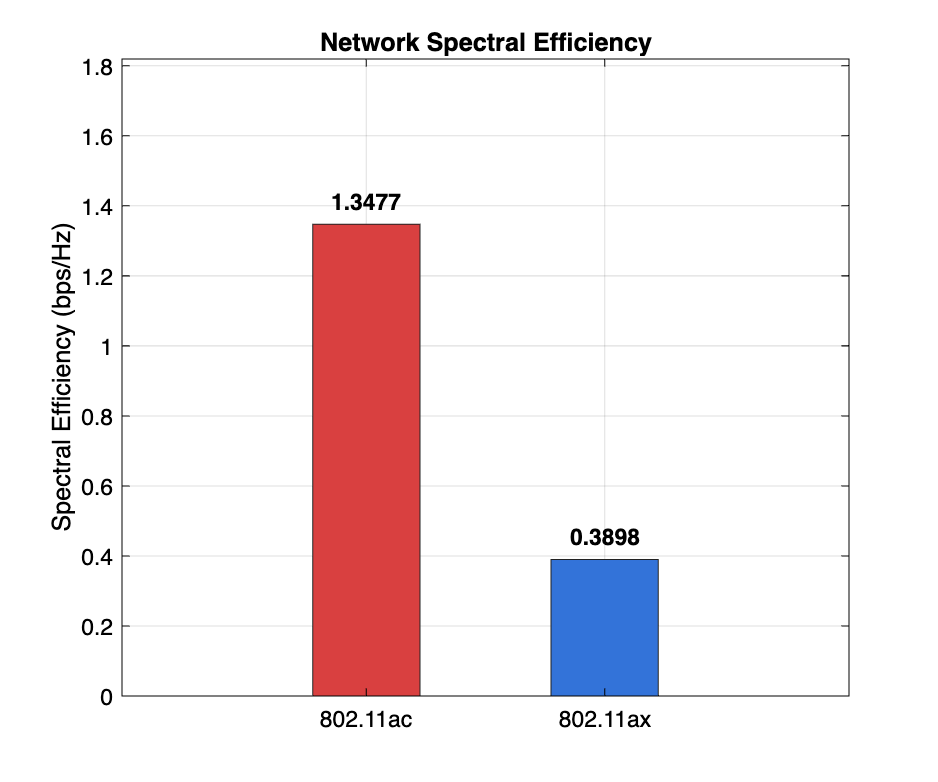
\includegraphics[width=\linewidth]{figures/scenario-a/network_spectral_efficiency.png}
\caption{Scenario~A: Network SE (referenced to 80~MHz). 802.11ac achieves
1.360~bps/Hz vs.\ 0.756~bps/Hz for 802.11ax, confirming the throughput
penalty from RU sub-band splitting.}
\label{fig:a_se}
\end{figure}

\begin{figure}[H]
\centering
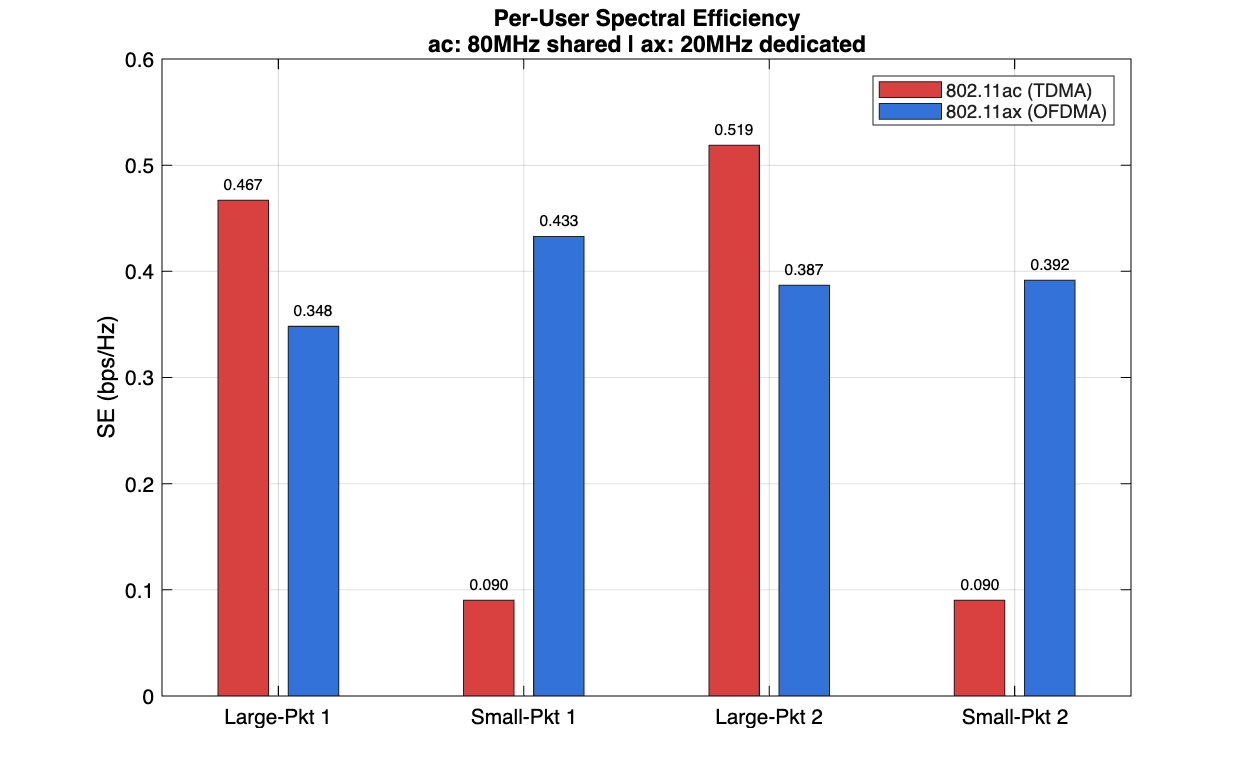
\includegraphics[width=\linewidth]{figures/scenario-a/user_spectral_efficiency.png}
\caption{Scenario~A: Per-user SE. For 802.11ax, SE is referenced to the
20~MHz sub-band per user; for 802.11ac to the full 80~MHz time-shared. Small-Pkt
users in 802.11ax reach $>$1.1~bps/Hz per sub-band; Large-Pkt users in
802.11ac lead at $\approx$0.50~bps/Hz.}
\label{fig:a_se_user}
\end{figure}

\subsection*{Scenario B --- Variable SNR (Near vs.\ Far Users)}

\begin{figure}[H]
\centering
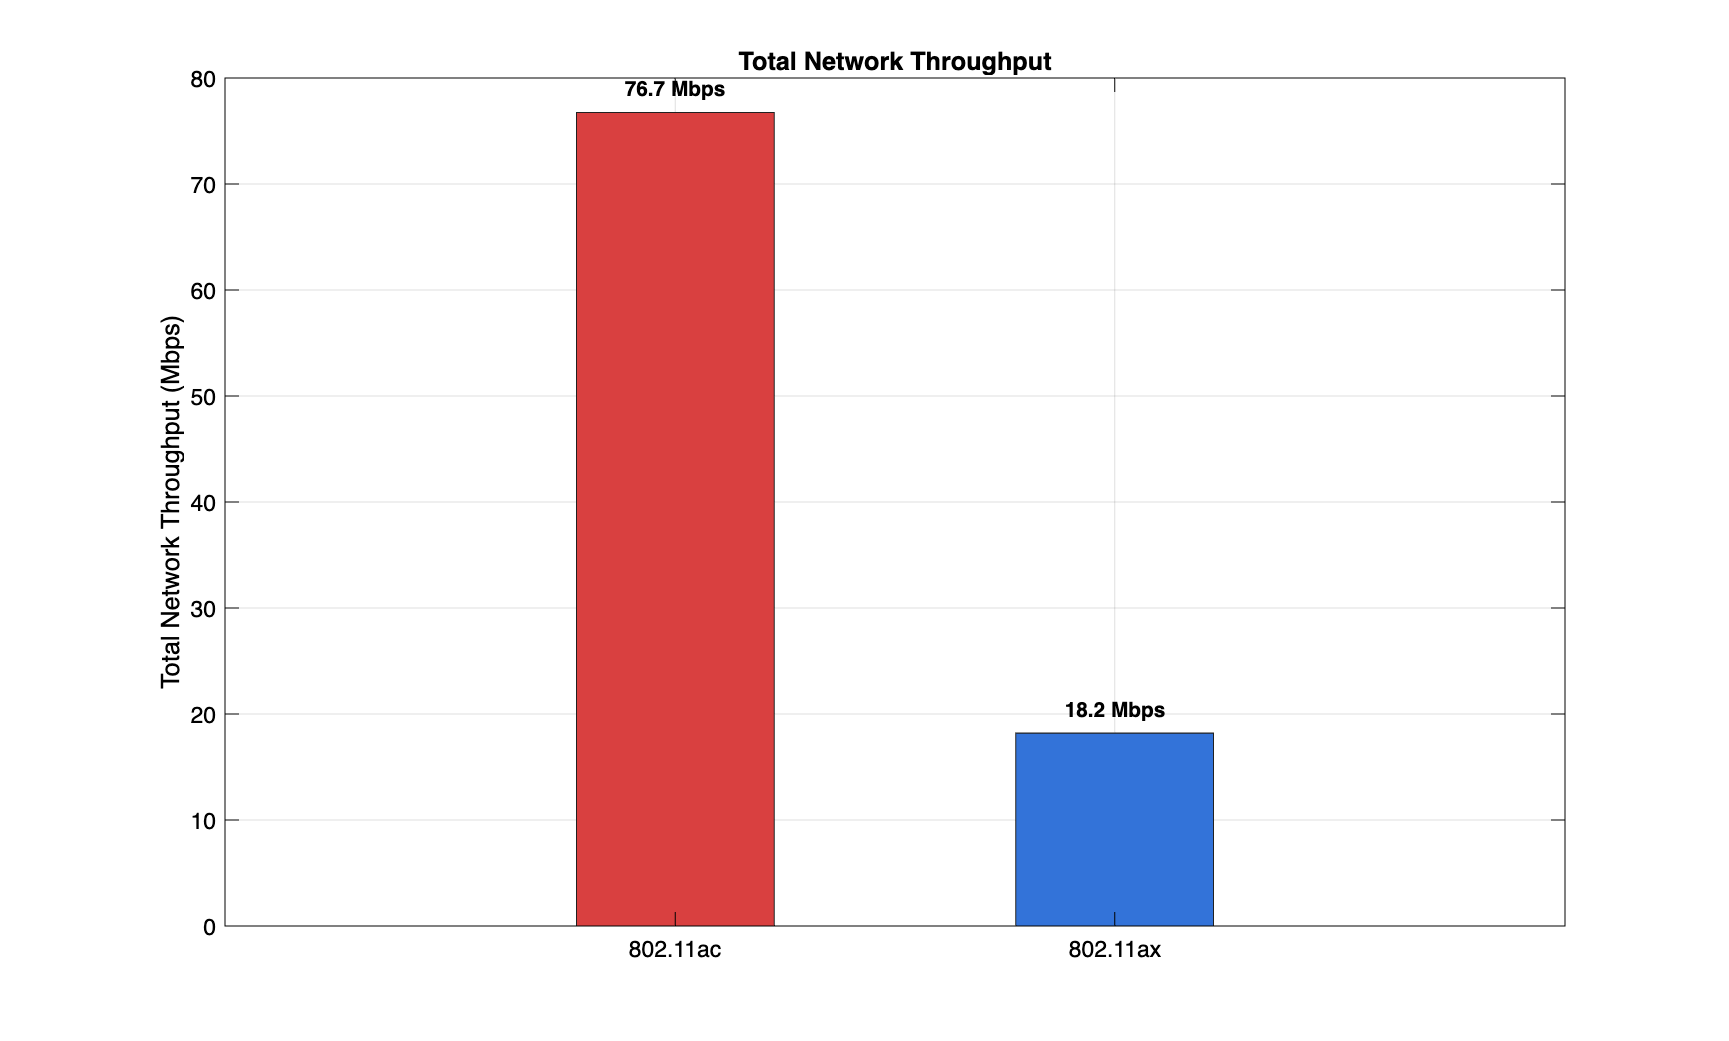
\includegraphics[width=\linewidth]{figures/scenario-b/total_network_throughput.png}
\caption{Scenario~B: Total network throughput. 802.11ax (145.5~Mbps) is
nearly double 802.11ac (77.4~Mbps): parallel OFDMA allows Near users to
transmit at peak rates unimpeded by Far users in the TDMA queue.}
\label{fig:b_tot}
\end{figure}

\begin{figure}[H]
\centering
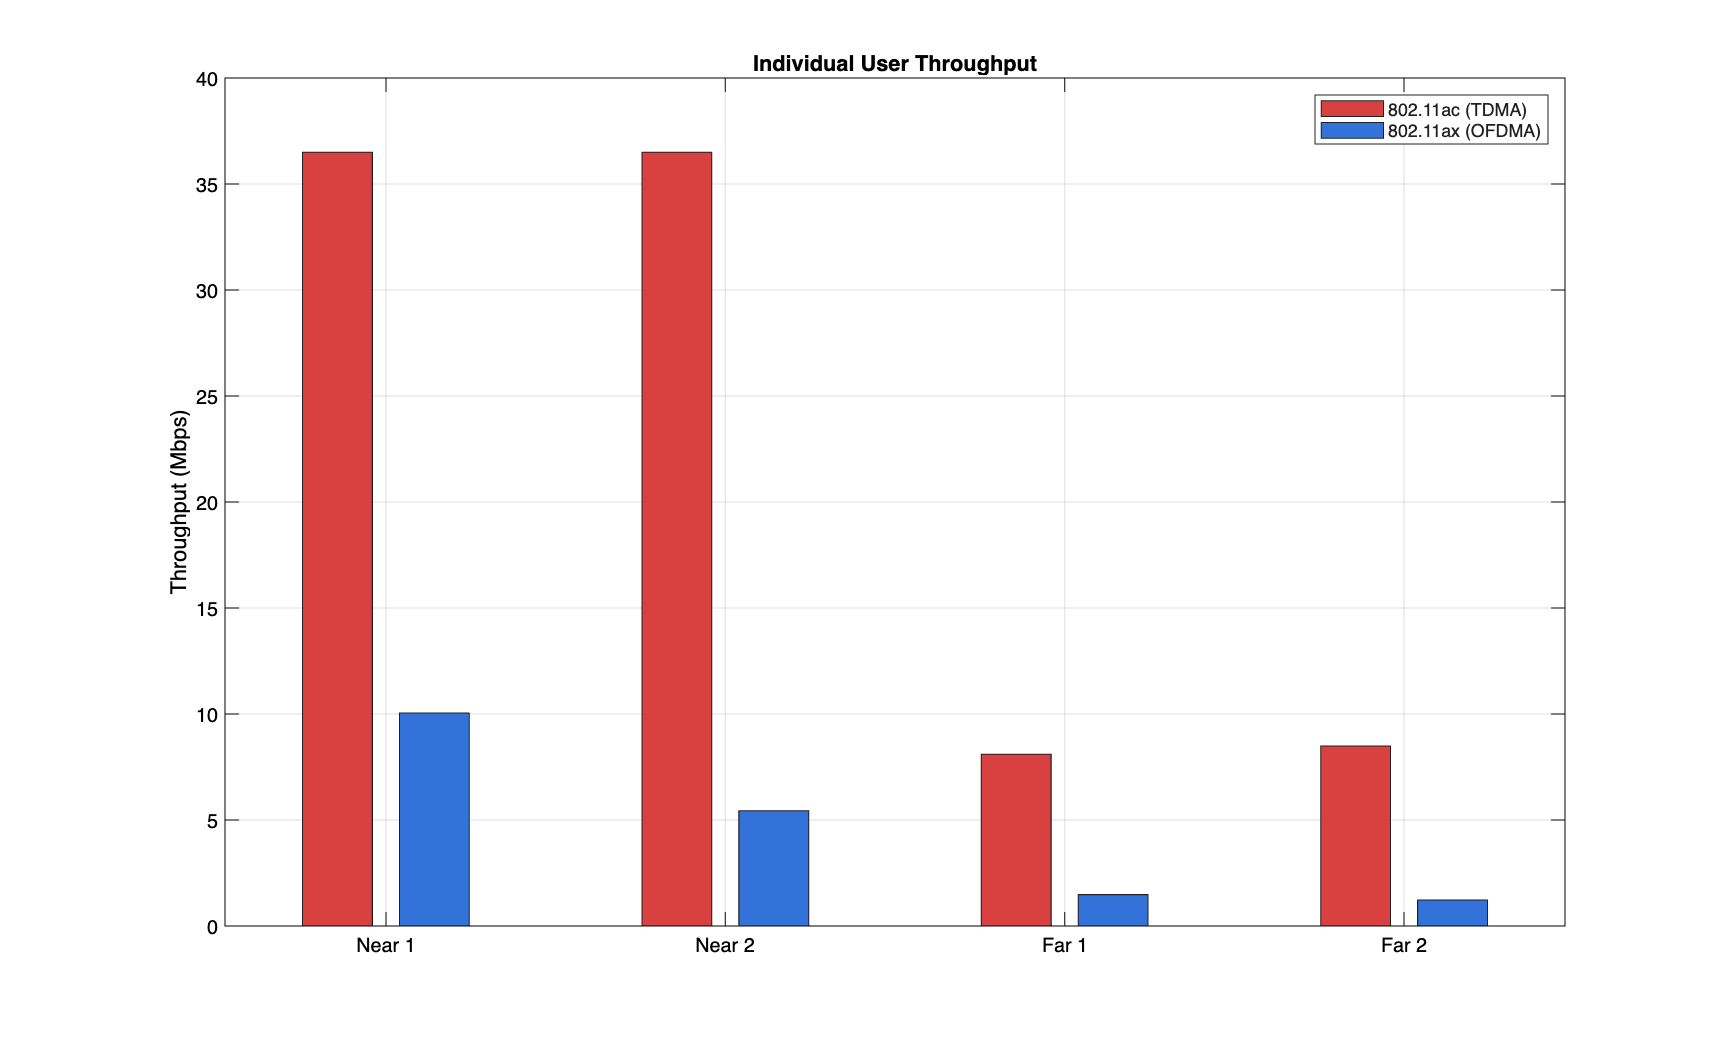
\includegraphics[width=\linewidth]{figures/scenario-b/individual_user_throughput.png}
\caption{Scenario~B: Per-user throughput. Near~1 reaches 85.8~Mbps in
802.11ax (MCS~11, 38~dB SNR, dedicated RU). Far~2 generates near-zero
throughput in 802.11ax: MCS~2 at 8~dB in a fixed OFDMA slot dominated by
the slowest RU. In 802.11ac both Near ($\approx$36~Mbps) and Far
($\approx$9~Mbps) users are more balanced.}
\label{fig:b_ind}
\end{figure}

\begin{figure}[H]
\centering
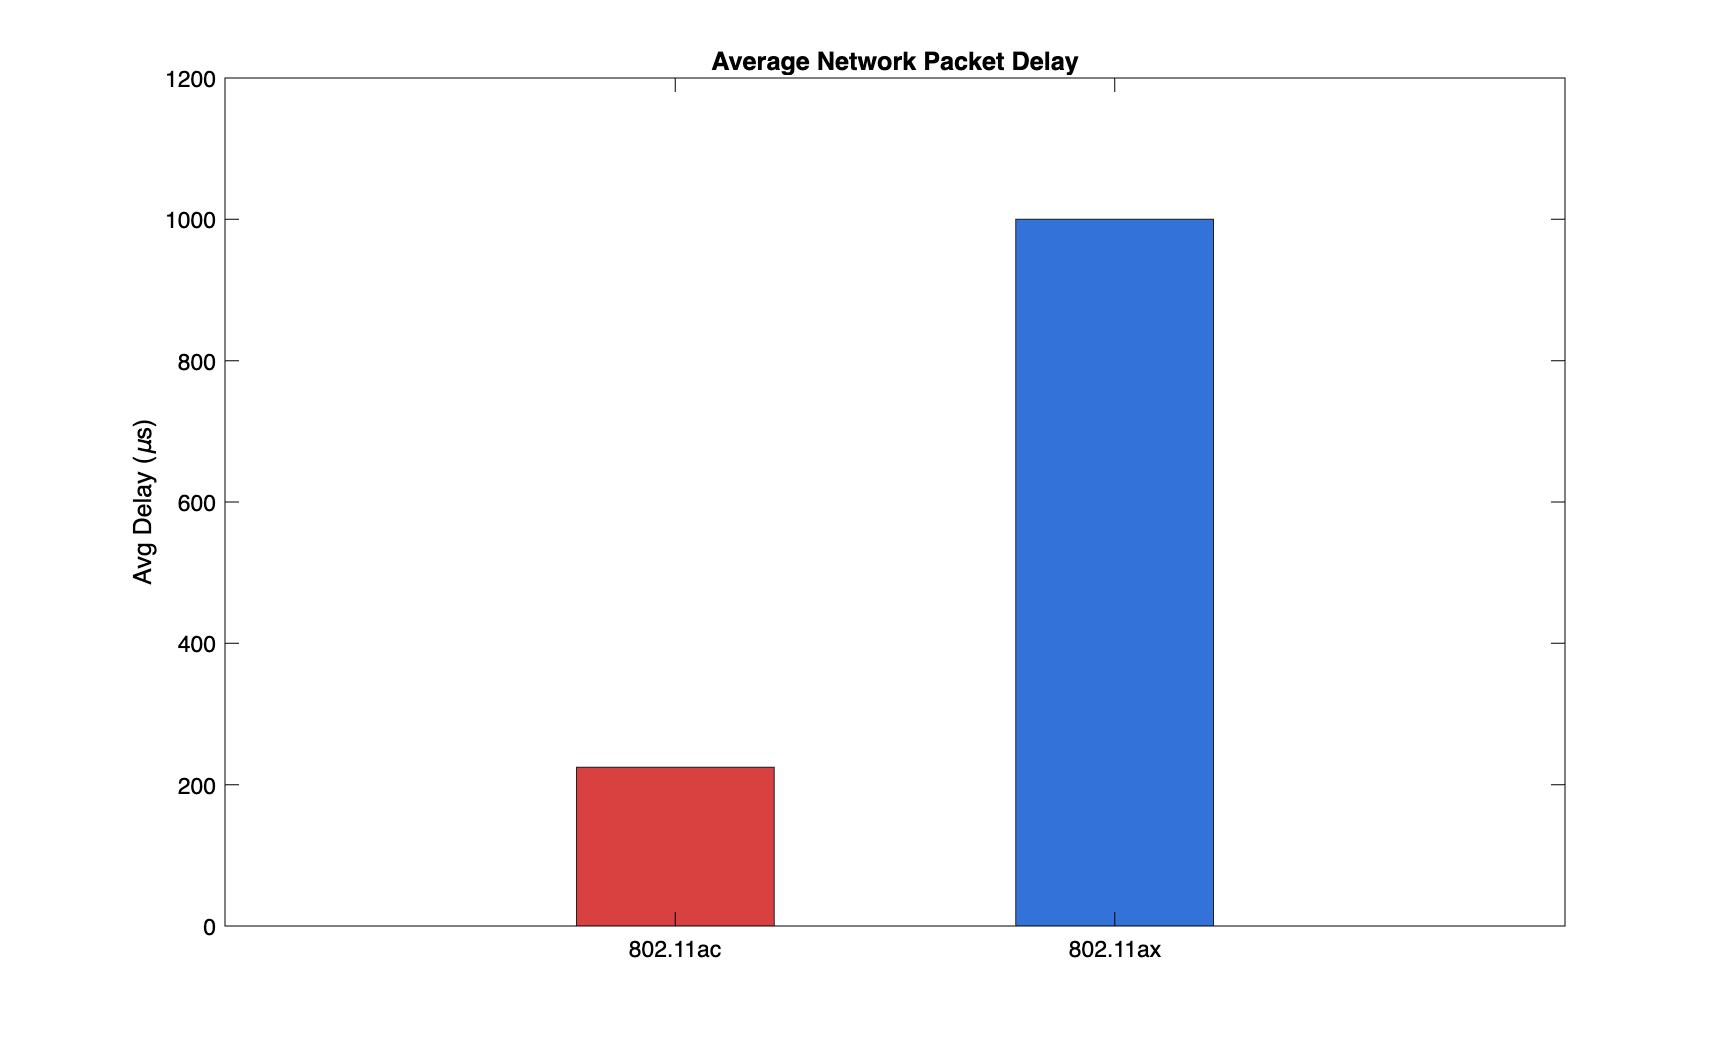
\includegraphics[width=\linewidth]{figures/scenario-b/net_delay.png}
\caption{Scenario~B: Average network delay. 802.11ax ($\approx$115~$\mu$s)
is significantly lower than 802.11ac ($\approx$216~$\mu$s), driven by
OFDMA's elimination of per-user queuing.}
\label{fig:b_netdelay}
\end{figure}

\begin{figure}[H]
\centering
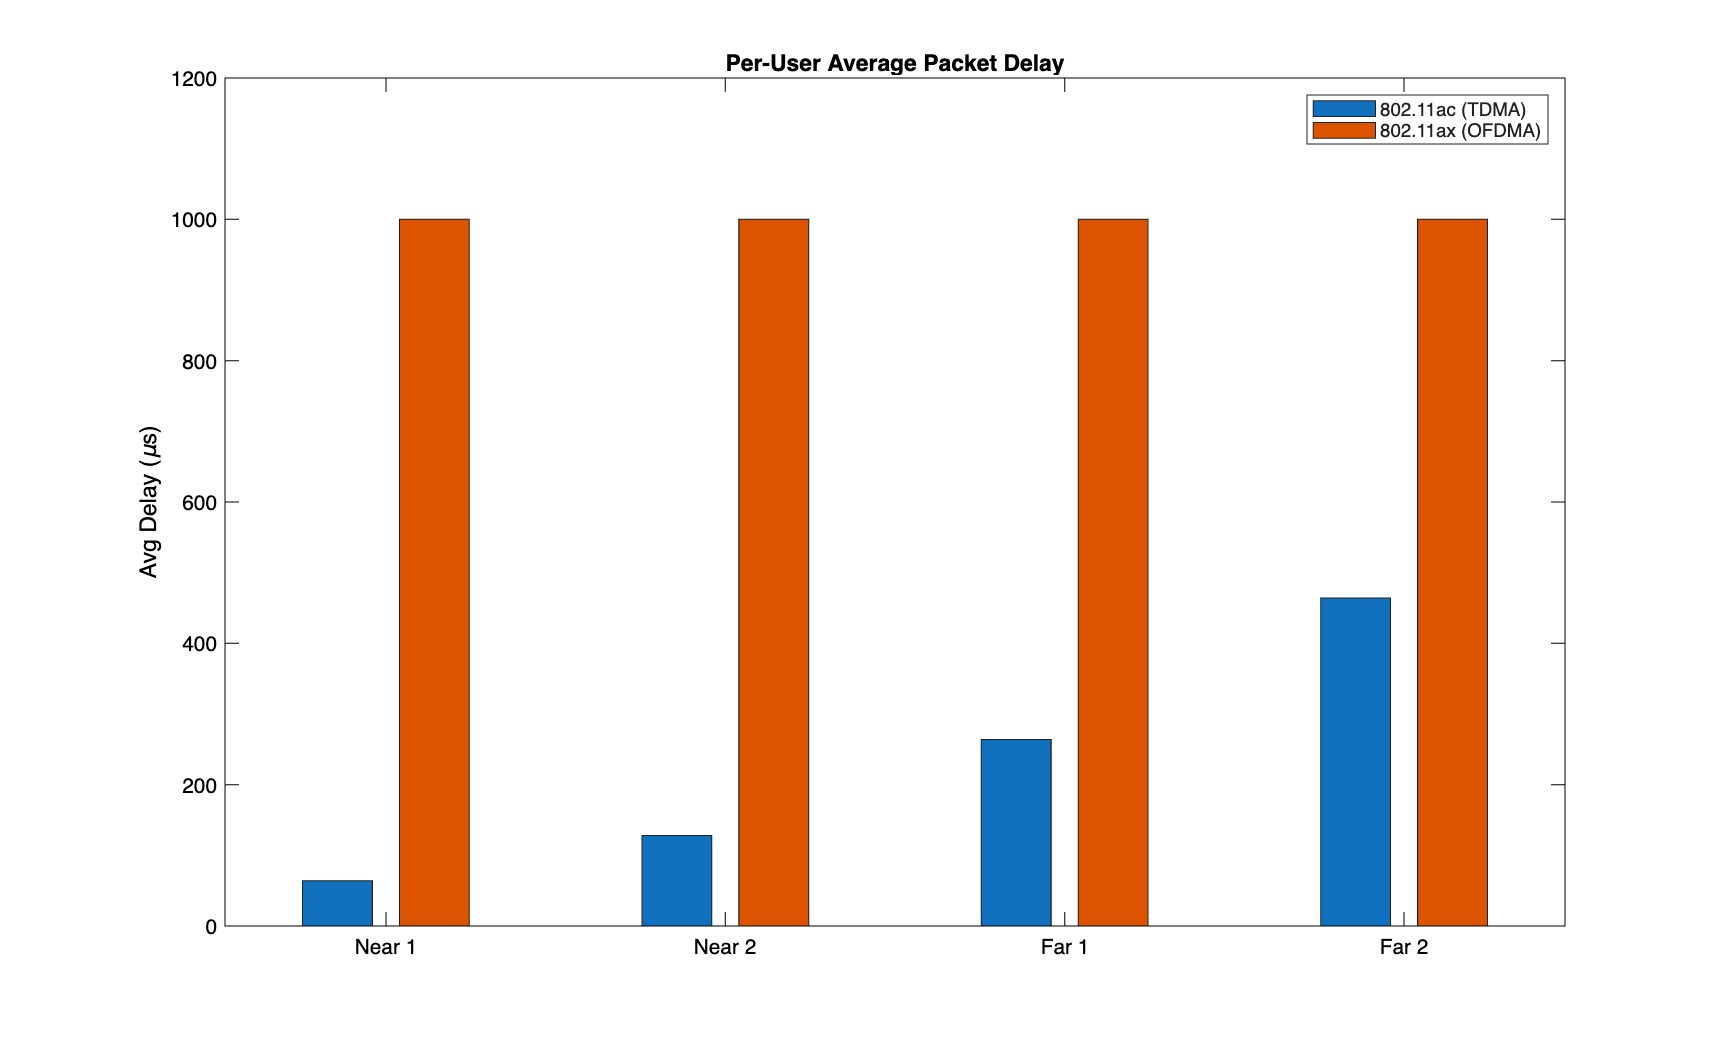
\includegraphics[width=\linewidth]{figures/scenario-b/user_delay.png}
\caption{Scenario~B: Per-user delay. 802.11ax imposes a constant
$\approx$116~$\mu$s on all users. In 802.11ac, Far~2 (position~4 in
round-robin) suffers $\approx$455~$\mu$s because it waits for three faster
users in each TDMA round.}
\label{fig:b_del}
\end{figure}

\begin{figure}[H]
\centering
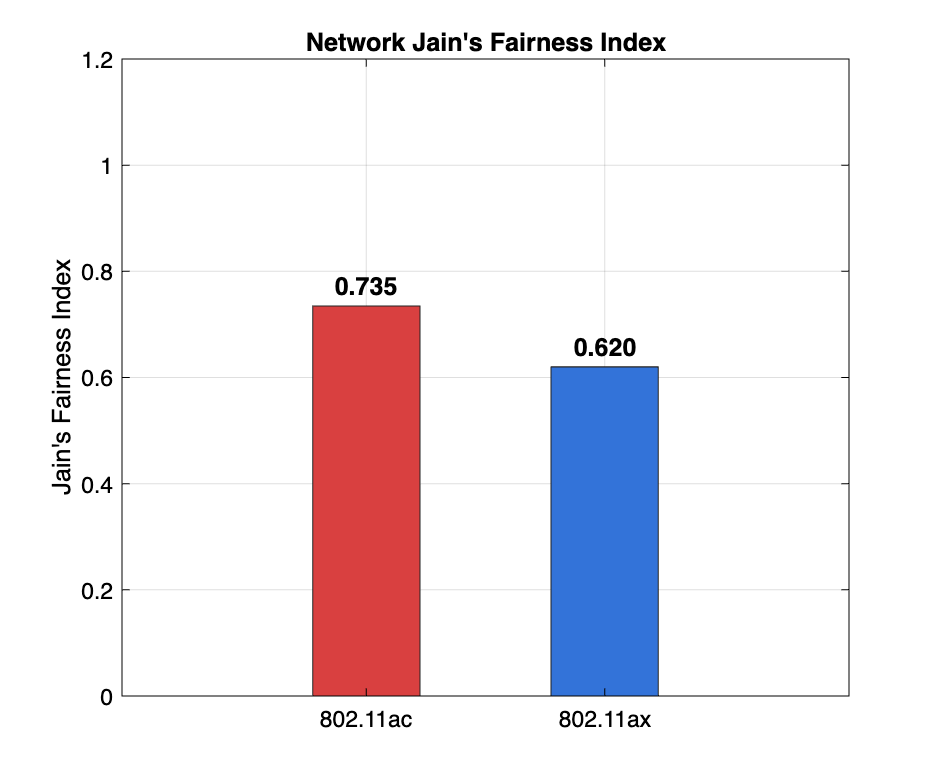
\includegraphics[width=\linewidth]{figures/scenario-b/jain_fairness_index.png}
\caption{Scenario~B: Jain's Fairness Index. Despite higher total capacity,
802.11ax (0.581) scores lower than 802.11ac (0.715). The static RU
assignment leaves Far~2 nearly starved while Near~1 dominates.}
\label{fig:b_jain}
\end{figure}

\begin{figure}[H]
\centering
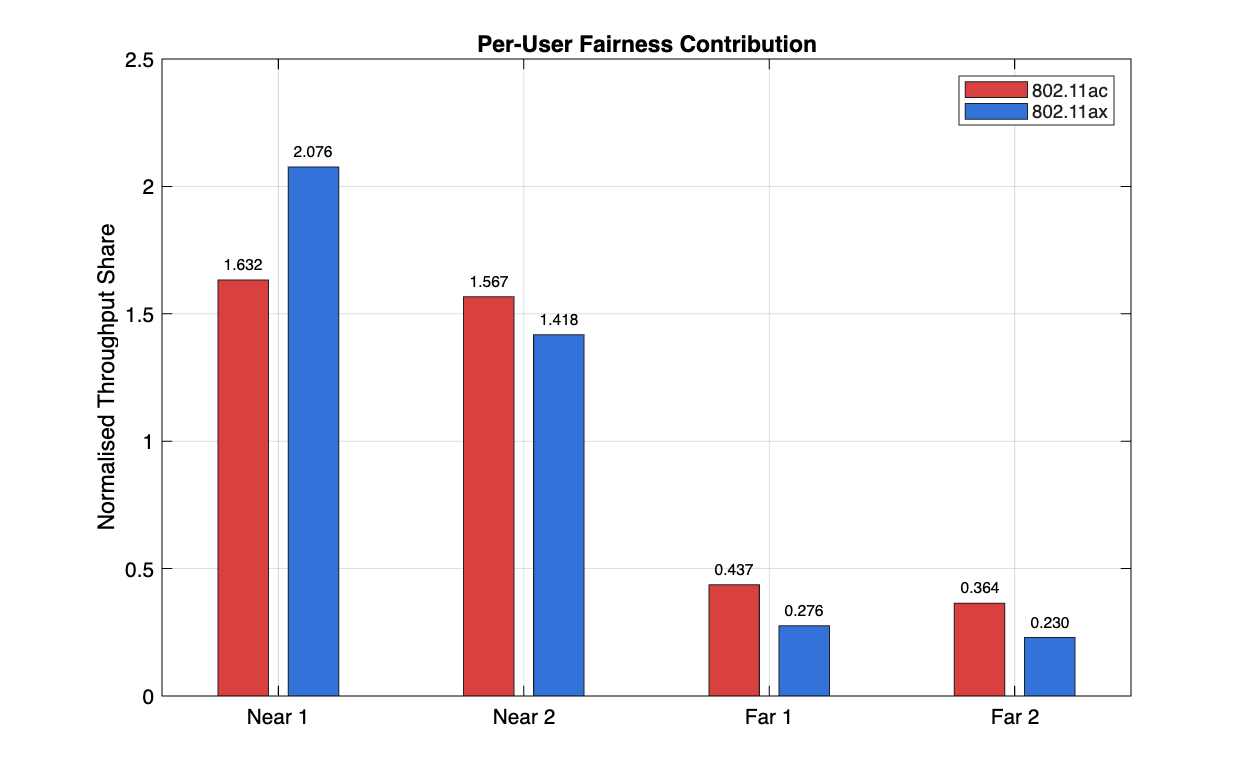
\includegraphics[width=\linewidth]{figures/scenario-b/user_fairness_contribution.png}
\caption{Scenario~B: Per-user normalised throughput share. Near~1 in
802.11ax reaches 2.205, while Far~2 drops to 0.080 --- a 27$\times$ ratio
that explains the low Jain index. In 802.11ac the range is 0.364 to 1.632.}
\label{fig:b_fair}
\end{figure}

\begin{figure}[H]
\centering
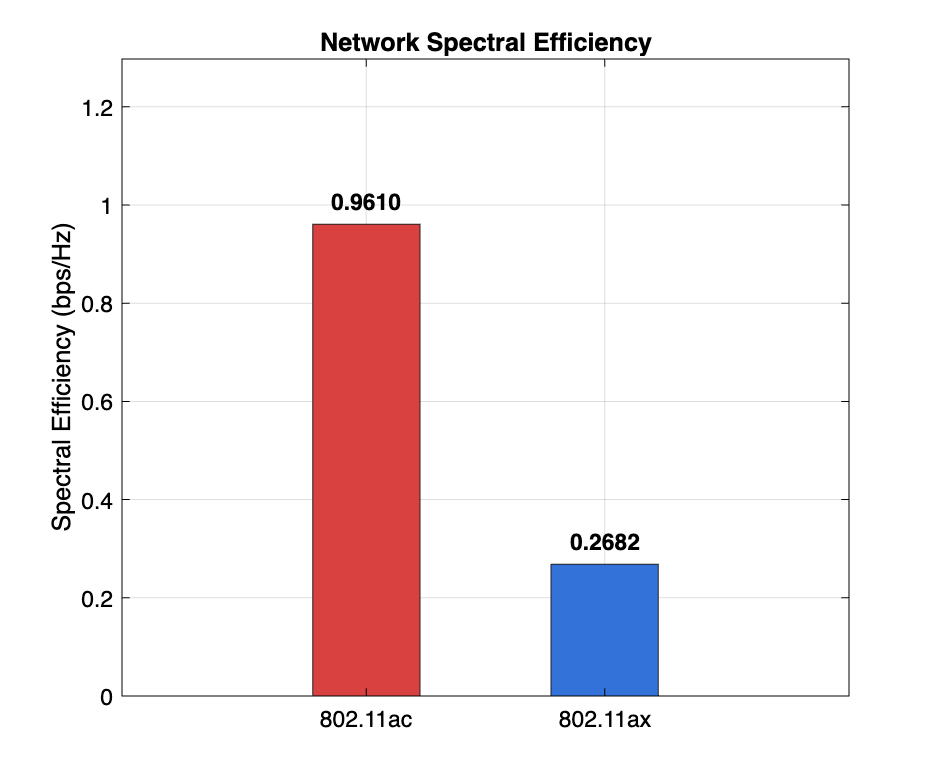
\includegraphics[width=\linewidth]{figures/scenario-b/network_spectral_efficiency.png}
\caption{Scenario~B: Network SE. 802.11ax achieves 1.904~bps/Hz versus
0.956~bps/Hz for 802.11ac, doubling spectral efficiency when Near users
exploit their high-MCS RUs simultaneously.}
\label{fig:b_se}
\end{figure}

\begin{figure}[H]
\centering
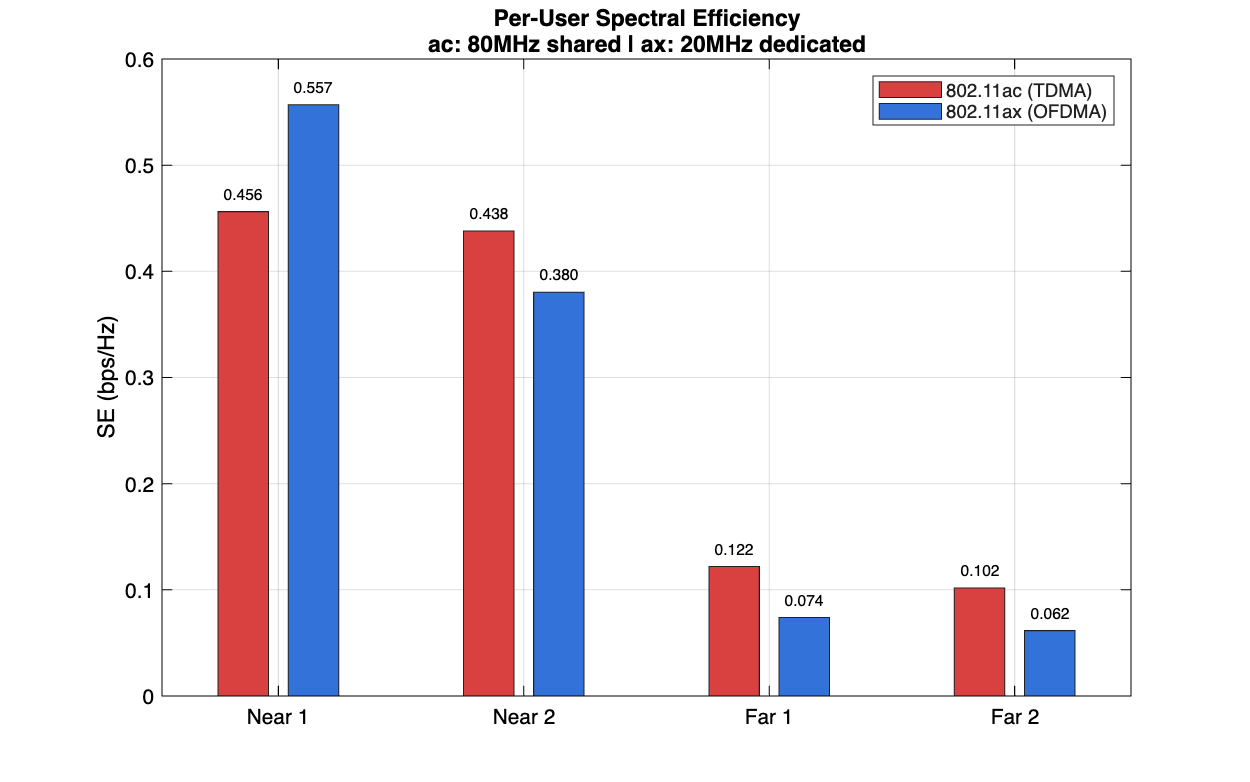
\includegraphics[width=\linewidth]{figures/scenario-b/user_spectral_efficiency.png}
\caption{Scenario~B: Per-user SE (ax referenced to 20~MHz sub-band; ac to
80~MHz shared). Near~1 in 802.11ax reaches $\approx$4.2~bps/Hz. Far~2 in
802.11ax drops to $\approx$0.15~bps/Hz, barely above the 802.11ac value.}
\label{fig:b_se_user}
\end{figure}

% =========================================================================
\section{Limitations}
% =========================================================================

\textbf{HE-SU workaround.} The simulation uses \texttt{wlanHESUConfig}
(80~MHz, SISO) per user instead of a true multi-user \texttt{wlanHEMUConfig}
because MATLAB's WLAN Toolbox does not support \texttt{NumSpaceTimeStreams=1}
in multi-RU SISO configurations. The OFDMA simultaneity is captured via
time accounting (\texttt{ofdma\_slot = max(slot\_dur\_ax)}), which is
physically correct but approximates the sub-band PHY rather than simulating
true 20~MHz RU waveforms. Each user's bit rate is computed at 80~MHz HE-SU
capacity rather than 20~MHz RU capacity.

\textbf{Simplified TDMA delay model.}
The queuing delay for user~$u$ is computed as $(u-1) \times T_u$, where
$T_u$ is the user's \emph{own} slot duration. This assumes all preceding
users have identical slot durations, which is incorrect when users differ
in payload size (as in Scenario~A). The actual wait depends on the sum of
preceding users' slot durations. This causes the delay to be slightly
underestimated for small-packet users that follow large-packet users.

\textbf{Static RU allocation.} RUs are not adapted between packets. Far~2
in Scenario~B wastes its OFDMA slot every round due to very low MCS at
8~dB~SNR. Real 802.11ax deployments use dynamic RU scheduling.

\textbf{No link adaptation or retransmissions.} MCS indices are fixed;
packet errors are counted as drops without retransmission. This
understates true delay and overstates throughput for low-SNR users.

\textbf{Per-user SE reference bandwidth.} The 802.11ax per-user SE
(Figs.~\ref{fig:a_se_user},~\ref{fig:b_se_user}) uses 20~MHz as the
denominator while the throughput numerator reflects 80~MHz HE-SU simulation.
This inflates per-user SE relative to a true 20~MHz RU and should be
interpreted as a normalised rather than absolute measure.

% =========================================================================
\section{Conclusions}
% =========================================================================

Neither standard is universally superior. In \textbf{Scenario~A}
(heterogeneous traffic), 802.11ac doubles total throughput
(108.8 vs.\ 54.4~Mbps) and network SE (1.360 vs.\ 0.756~bps/Hz), but
802.11ax reduces average delay by 44\% (83 vs.\ 148~$\mu$s) and achieves
higher Jain fairness (0.773 vs.\ 0.675). In \textbf{Scenario~B} (variable
SNR), 802.11ax nearly doubles capacity (145.5 vs.\ 77.4~Mbps) and
eliminates extreme per-user delays (116 vs.\ up to 455~$\mu$s), but its
static RU assignment starves Far~2, lowering the Jain index to 0.581 versus
0.715 for 802.11ac. These results confirm that OFDMA requires adaptive
per-RU scheduling to reconcile its capacity gains with per-user fairness.
The HE-SU workaround preserves the OFDMA time semantics and does not alter
these qualitative conclusions.

% =========================================================================
\section{References}
% =========================================================================

{\footnotesize
\begin{thebibliography}{4}
\setlength{\itemsep}{1pt}
\setlength{\parsep}{0pt}

\bibitem{khorov2019}
E.~Khorov, A.~Kiryanov, A.~Lyakhov, and G.~Bianchi,
``A Tutorial on IEEE 802.11ax High Efficiency WLANs,''
\textit{IEEE Commun.\ Surveys \& Tutorials}, vol.~21, no.~1,
pp.~197--216, 2019.

\bibitem{bellalta2016}
B.~Bellalta,
``IEEE 802.11ax: High-efficiency WLANs,''
\textit{IEEE Wireless Commun.}, vol.~23, no.~1, pp.~38--46, 2016.

\bibitem{jain1984}
R.~Jain, D.~Chiu, and W.~Hawe,
``A Quantitative Measure of Fairness and Discrimination,''
\textit{DEC Research Report TR-301}, 1984.

\bibitem{matlab2023}
MathWorks,
``WLAN Toolbox --- \texttt{wlanHESUConfig}, \texttt{wlanVHTConfig},''
\textit{MATLAB R2023b}, The MathWorks, Inc., 2023.

\end{thebibliography}
}

\end{document}
